%\section*{Phase 1: 1.0 Business Understanding}

\subsection*{Task 1.1: Determine Business Objectives}
%\subsubsection*{Deliverable: Project Scope Document -- Part 1}

The primary objective of this project is to support real estate investors and property managers operating in the Southern USA by identifying which apartment amenities most significantly influence rental price. Understanding amenity importance enables strategic property improvements and competitive pricing decisions in high-growth Southern markets.

\medskip\noindent
\textbf{Target Audience}
\vspace{-9pt}
\begin{itemize}[itemsep=-9pt]
    \item Real estate investors seeking to maximize return on amenity upgrades
    \item Property managers aiming to set competitive rental prices relative to local Southern market conditions
\end{itemize}

\vspace{-9pt}
%\medskip
\noindent
\textbf{Business Questions}
\vspace{-9pt}
\begin{itemize}[itemsep=-9pt]
    \item Which amenities have the strongest impact on rental pricing?
    \item How does amenity importance vary across geographic regions?% (Austin vs. Miami vs. Atlanta)?
    \item Which amenity upgrades yield the highest price premium relative to cost?
    \item Do certain amenity bundles (e.g., parking and laundry) have compounding effects on price?
\end{itemize}

\vspace{-9pt}
%\medskip
\noindent
\textbf{Success Criteria}

The project succeeds when a model can identify the top amenity drivers of rental price, producing rankings that are actionable for renovation prioritization and pricing strategy in Southern apartment markets.

\subsection*{Task 1.2: Assess the Situation}
%\subsubsection*{Deliverable: Project Scope Document -- Part 2}

\noindent
\textbf{Stakeholder Analysis}

Investors and property managers share a common anchor: understanding what drives property value. Investors seek to maximize return on capital allocated to amenity upgrades. Property managers need to price units competitively against comparable listings in the same Southern city. Both groups benefit from a clear, ranked understanding of which amenities move rental price.

\medskip\noindent
\textbf{Data Source and Inventory}

The dataset was sourced from Kaggle (Craigslist scrape, January 2020): 384,977 rows, 22 columns, 558 MB. The target variable is \texttt{price} (monthly rental price in USD). Features include square footage, bedroom and bathroom counts, geographic coordinates, and categorical amenity flags (parking, laundry, pet policies, wheelchair access, smoking policy, electric vehicle charging, furnished status).

\medskip\noindent
\textbf{Constraints}
\vspace{-9pt}
\begin{itemize}[itemsep=-9pt]
    \item Dataset reflects 2020 market conditions; no real-time pricing data is available
    \item No GPU or TPU hardware available, which limits NLP analysis of the listing description% field
    \item Geographic scope is restricted to Southern states %6 Southern cities: Austin TX, Dallas TX, Miami FL, Atlanta GA, Nashville TN, and Charlotte NC
\end{itemize}

\vspace{-9pt}
%\medskip
\noindent
\textbf{Risks and Contingencies}
\vspace{-9pt}
\begin{itemize}[itemsep=-9pt]
    \item \textit{Missing values:} public listing data commonly contains incomplete amenity fields%(e.g., laundry, parking options) and missing geographic coordinates; 
    ; plan to %impute missing categoricals as a dedicated category and 
    exclude records with unusable location data.
    \item \textit{Anomalous records:} listing platforms may include erroneous entries (e.g., zero-price listings, implausible square footage); plan to apply threshold-based filters before modeling
    \item \textit{Outlier contamination:} regional price distributions in diverse Southern markets may be skewed by extreme listings; plan to apply outlier removal at the state/region level %rather than nationally
\end{itemize}

\subsection*{Task 1.3: Determine Data-Mining Goals}
%\subsubsection*{Deliverable: Data-Mining Scope Document}

The data-mining goals for this project are twofold:
\vspace{-12pt}
\begin{itemize}[itemsep=-9pt]
    \item \textbf{Predictive goal:} predict apartment rental price using all available features in the dataset
    \item \textbf{Analytical goal:} determine the relative importance of each amenity feature in driving the predicted price, producing an actionable ranking for investors and property managers
\end{itemize}

\medskip\noindent
\textbf{Modeling Strategy}

Three tree-based ensemble methods are used: Random Forest, Gradient Boosting, and XGBoost. Tree-based methods are selected because they handle mixed data types (numeric and categorical), are robust to outliers, and natively produce feature importance scores. A K-Means clustering step on latitude and longitude %(125 clusters) 
engineers a \texttt{location\_cluster} feature to capture local market effects beyond state-level geography.

\medskip\noindent
\textbf{Success Metrics}

Model performance is evaluated on a held-out 20\% test set using: Mean Absolute Error (MAE), Root Mean Squared Error (RMSE), R-squared (R\textsuperscript{2}), Average Squared Error (ASE), and Sum of Squared Errors (SSE).

\subsection*{Task 1.4: Produce a Project Plan}
%\subsubsection*{Deliverable: Data Mining Project/Resource Plan}

This project follows the CRISP-DM (Cross-Industry Standard Process for Data Mining) methodology across six structured phases: Business Understanding, Data Understanding, Data Preparation, Modeling, Evaluation, and Deployment. Each phase produces one or more formal deliverables submitted according to the course schedule.

\begin{center}
  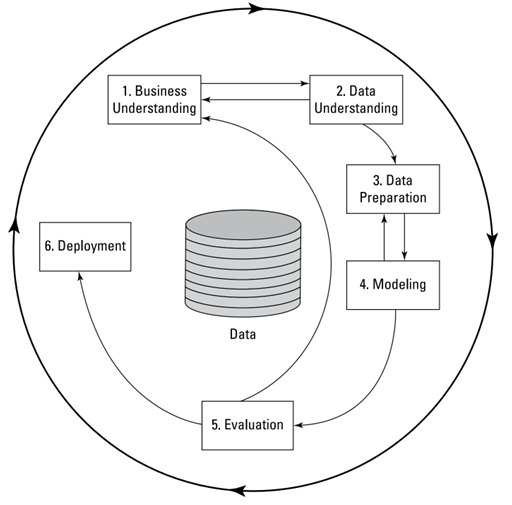
\includegraphics[height=150pt]{Assignment/week1/charts/CRISP-DM.png}\\[4pt]
  {\small\textit{Figure 1: CRISP-DM pipeline diagram}}
\end{center}

\medskip\noindent
\textbf{Tools and Hardware}

{\renewcommand{\arraystretch}{0.75}
\begin{center}
\begin{tabular}{ll}
\hline
\textbf{Category} & \textbf{Details} \\
\hline
Language / IDE & Python 3.12.3, VS Code, Jupyter Notebook \\
Key Libraries & pandas 3.0.1, numpy 2.4.2, matplotlib 3.10.8, scipy 1.17.1 \\
               & scikit-learn 1.8.0, xgboost 3.2.0, category-encoders 2.9.0, joblib 1.5.3 \\
Data Source    & \href{https://www.kaggle.com/datasets/austinreese/usa-housing-listings}{Kaggle} (Craigslist scrape, January 2020) \\
Hardware       & 2 vCPU, 2 GB RAM, Ubuntu 24 Server \\
\hline
\end{tabular}
\end{center}}%

\medskip\noindent
\textbf{Complete Project Timeline}

{\renewcommand{\arraystretch}{0.75}
\begin{center}
\begin{tabular}{lp{6.5cm}l}
\hline
\textbf{Task} & \textbf{Description} & \textbf{Submission} \\
\hline
1.1 & Determine Business Objectives  & 9 May 2026  \\
1.2 & Assess the Situation           & 9 May 2026  \\
1.3 & Determine Data-Mining Goals    & 9 May 2026  \\
1.4 & Produce a Project Plan         & 9 May 2026  \\
\hline
2.1 & Gather Data                    & 23 May 2026 \\
2.2 & Describe Data                  & 23 May 2026 \\
2.3 & Explore Data                   & 23 May 2026 \\
2.4 & Verify Data Quality            & 23 May 2026 \\
\hline
3.1 & Select Data                    & 6 Jun 2026  \\
3.2 & Clean Data                     & 6 Jun 2026  \\
3.3 & Construct Data                 & 6 Jun 2026  \\
3.4 & Integrate Data                 & 6 Jun 2026  \\
3.5 & Format Data                    & 6 Jun 2026  \\
\hline
    & Midterm Presentation           & 13 Jun 2026 \\
\hline
4.1 & Select Modeling Technique      & 20 Jun 2026 \\
4.2 & Generate Test Design           & 20 Jun 2026 \\
4.3 & Build Model                    & 20 Jun 2026 \\
4.4 & Assess Model                   & 20 Jun 2026 \\
\hline
5.1 & Evaluate Results               & 4 Jul 2026  \\
5.2 & Review Process                 & 4 Jul 2026  \\
5.3 & Determine Next Steps           & 4 Jul 2026  \\
\hline
6.1 & Plan Deployment                & 11 Jul 2026 \\
6.2 & Plan Monitoring                & 11 Jul 2026 \\
6.3 & Final Report and Presentation  & 1 Aug 2026  \\
6.4 & Review Project                 & 1 Aug 2026  \\
\hline
\end{tabular}
\end{center}}%
